\newpage
%================================================================
\section{Results and Discussion}\label{sec:Results}
%================================================================

\subsection{The effect of the latent dimension}  

\autoref{fig:loss_latent_dim_vanilla_vae_bmnist} show the ELBO ... during training for different choices of latent dimensions. In terms of the loss, the Conv-VAE generally performs slightly better than the MLP- and DNN-VAE.
why? cnn in principle better at extracting features 

\begin{figure}[!htb]
\begin{center}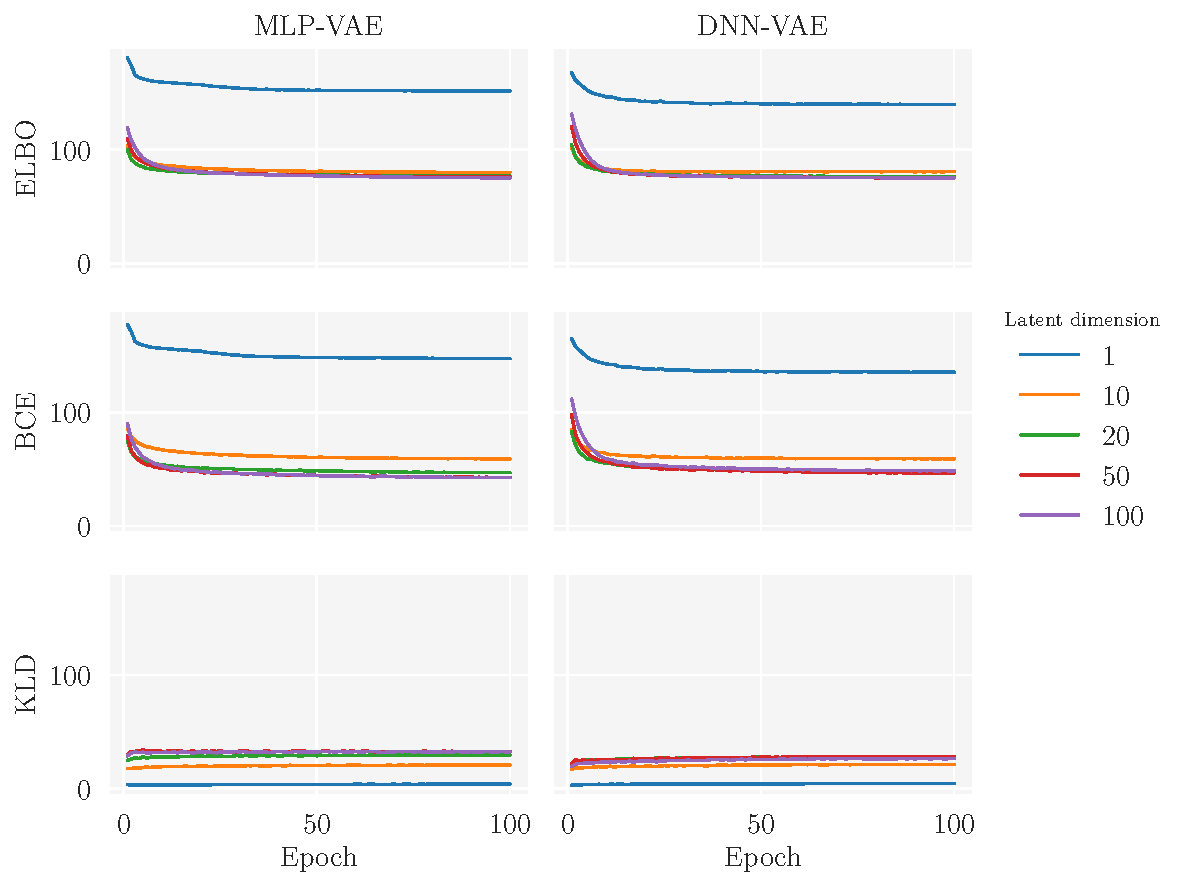
\includegraphics[scale=0.75]{latex/figures/loss_latent_dim_vanilla_mlp_dnn_vae_bmnist.pdf}
\end{center}
\caption{figure text}
\label{fig:loss_latent_dim_vanilla_vae_bmnist}
\end{figure}

\autoref{fig:recon_latent_dim_vanilla_vae_bmnist} shows the VAEs reconstructed images from the test set.

\begin{figure}[!htb]
\centering
\subfloat[]{{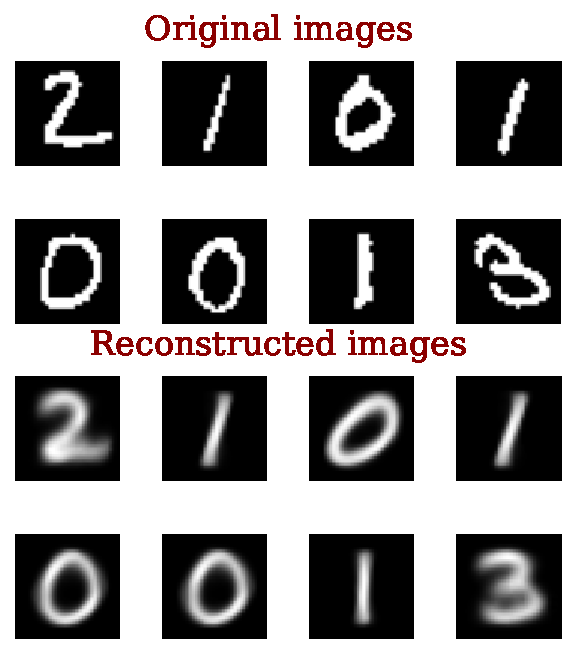
\includegraphics[scale=0.5]{latex/figures/recon_latent_dim_1_vanilla_mlp_vae_bmnist.pdf}}}
\qquad
\subfloat[]{{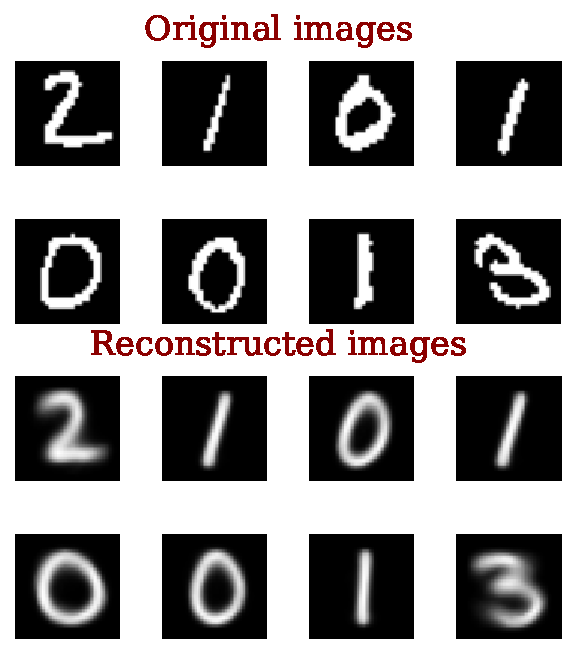
\includegraphics[scale=0.5]{latex/figures/recon_latent_dim_1_vanilla_dnn_vae_bmnist.pdf}}}
\qquad
\subfloat[]{{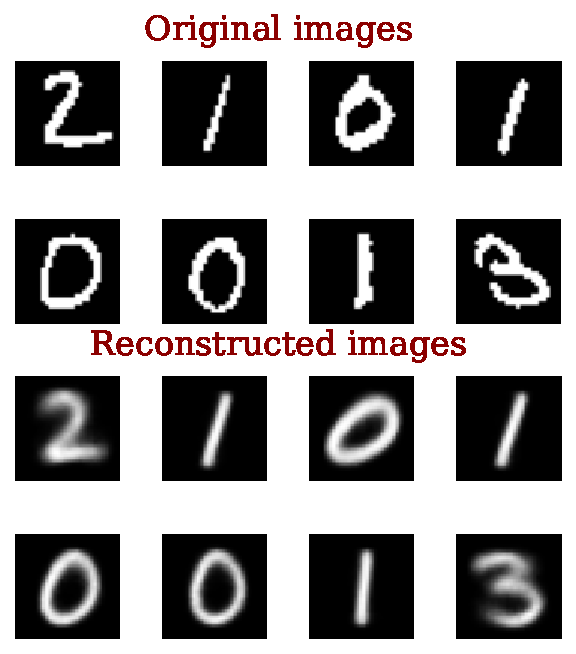
\includegraphics[scale=0.5]{latex/figures/recon_latent_dim_1_vanilla_conv_vae_bmnist.pdf}}}
\qquad
\subfloat[]{{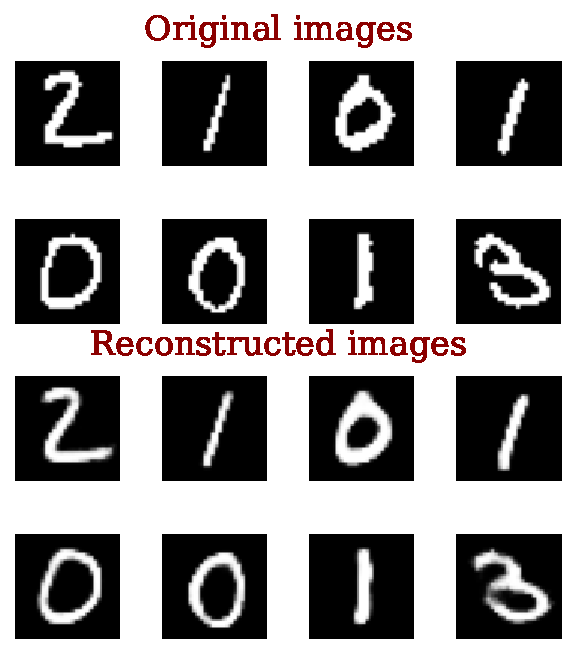
\includegraphics[scale=0.5]{latex/figures/recon_latent_dim_20_vanilla_mlp_vae_bmnist.pdf}}}
\qquad
\subfloat[]{{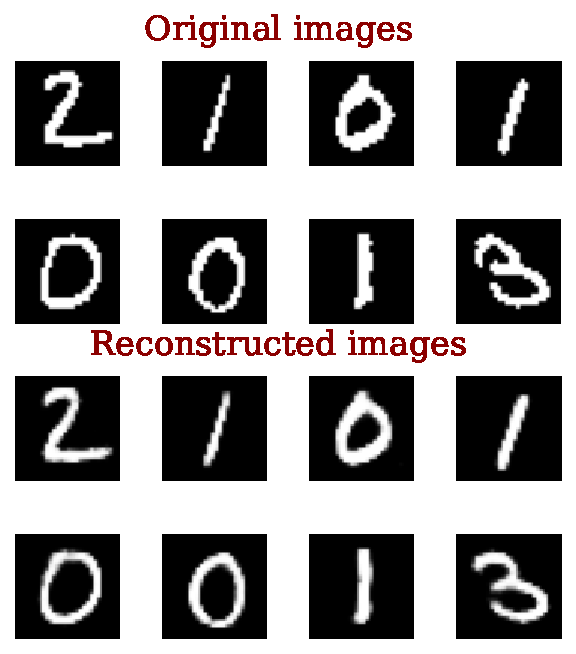
\includegraphics[scale=0.5]{latex/figures/recon_latent_dim_20_vanilla_dnn_vae_bmnist.pdf}}}
\qquad
\subfloat[]{{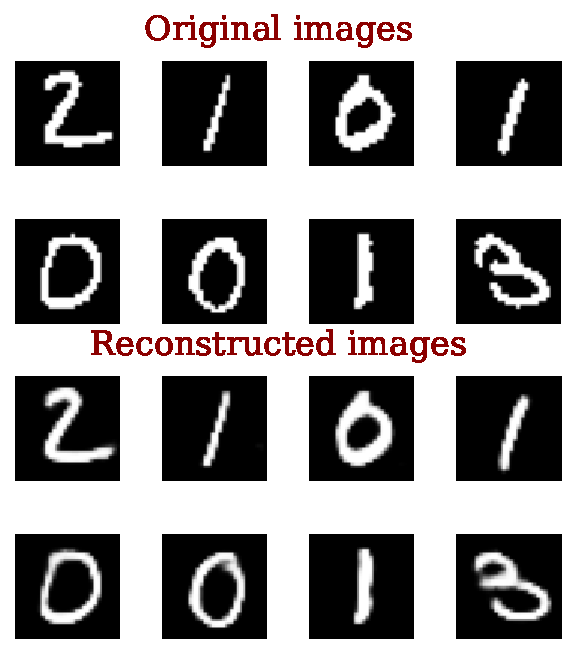
\includegraphics[scale=0.5]{latex/figures/recon_latent_dim_20_vanilla_conv_vae_bmnist.pdf}}}
\qquad
\subfloat[]{{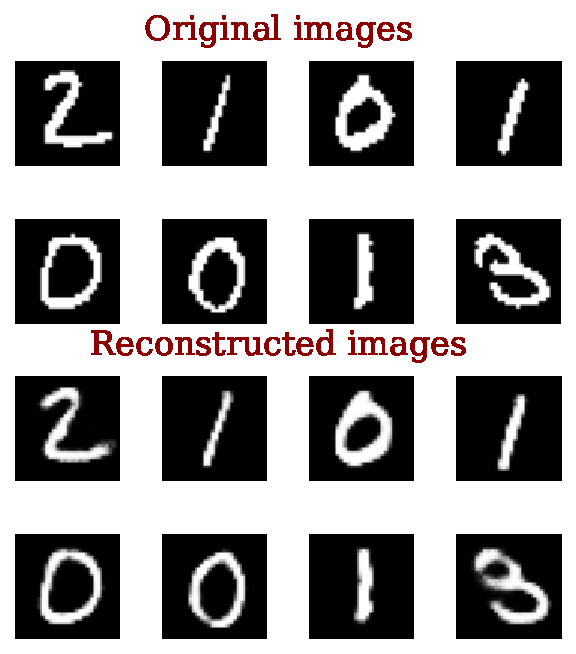
\includegraphics[scale=0.5]{latex/figures/recon_latent_dim_100_vanilla_mlp_vae_bmnist.pdf}}}
\qquad
\subfloat[]{{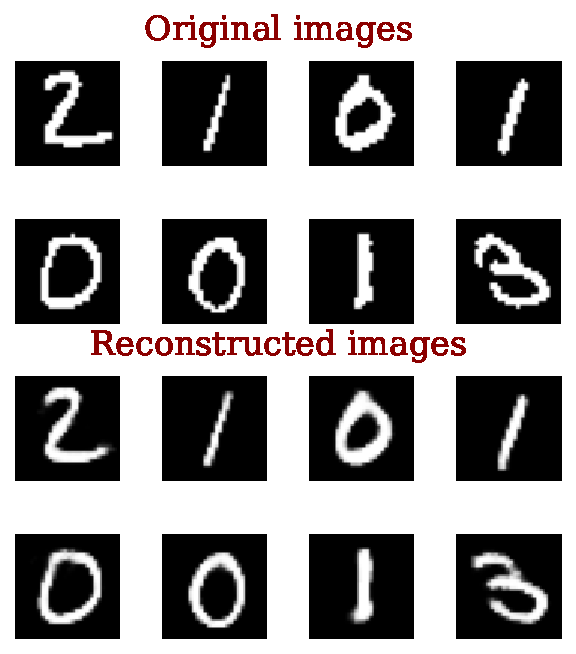
\includegraphics[scale=0.5]{latex/figures/recon_latent_dim_100_vanilla_dnn_vae_bmnist.pdf}}}
\qquad
\subfloat[]{{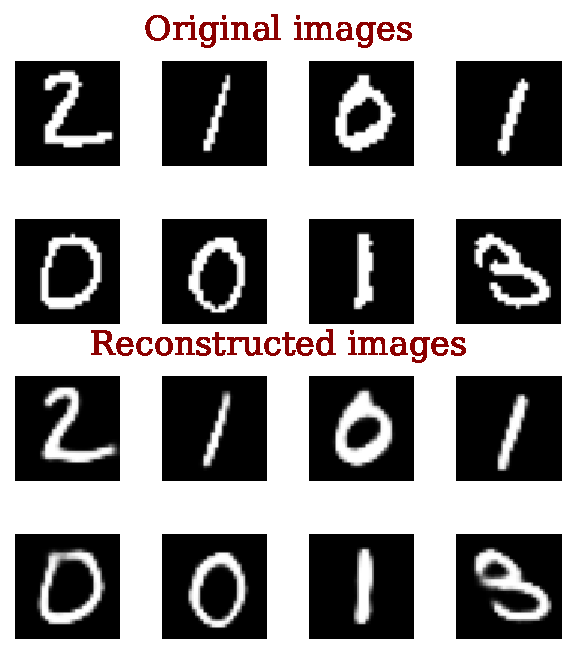
\includegraphics[scale=0.5]{latex/figures/recon_latent_dim_100_vanilla_conv_vae_bmnist.pdf}}}
\caption{Comparison of original and reconstructed images. Grids to the left are the MLP-VAE, in the middle DNN-VAE and to the right Conv-VAE. The top row shows 1 latent dimension, the middle 20 latent dimensions and the bottom 100}
\label{fig:recon_latent_dim_vanilla_vae_bmnist}
\end{figure}


\autoref{fig:samples_latent_dim_vanilla_vae_bmnist} shows generated samples

\begin{figure}[!htb]
\centering
\subfloat[]{{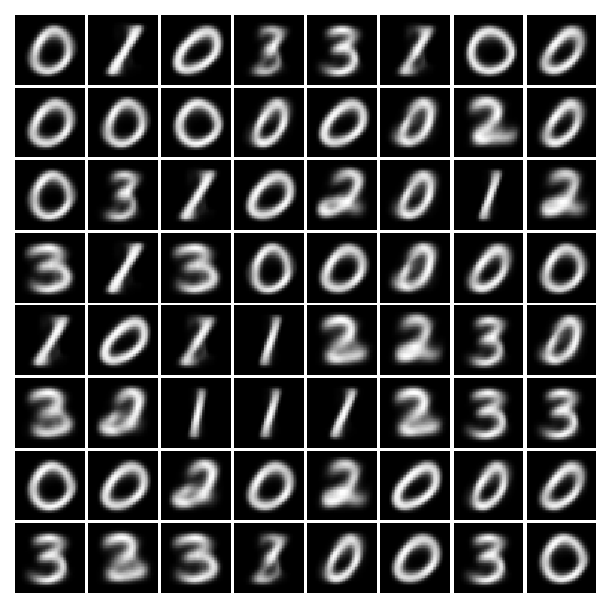
\includegraphics[scale=0.45]{latex/figures/samples_latent_dim_1_vanilla_mlp_vae_bmnist.pdf}}}
\qquad
\subfloat[]{{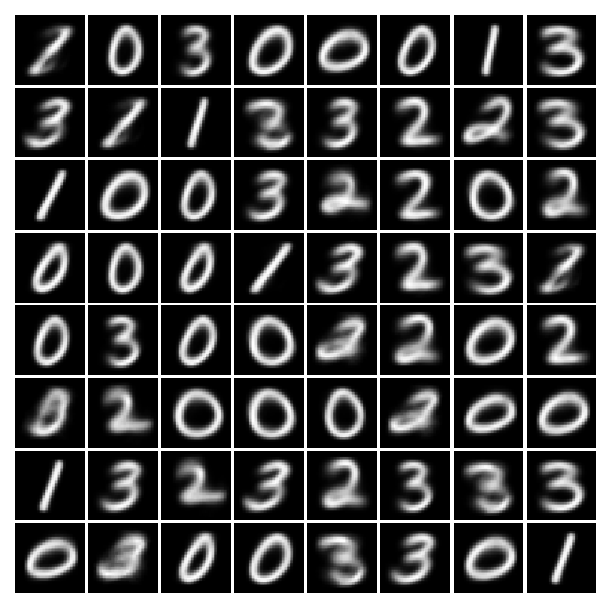
\includegraphics[scale=0.45]{latex/figures/samples_latent_dim_1_vanilla_dnn_vae_bmnist.pdf}}}
\qquad
\subfloat[]{{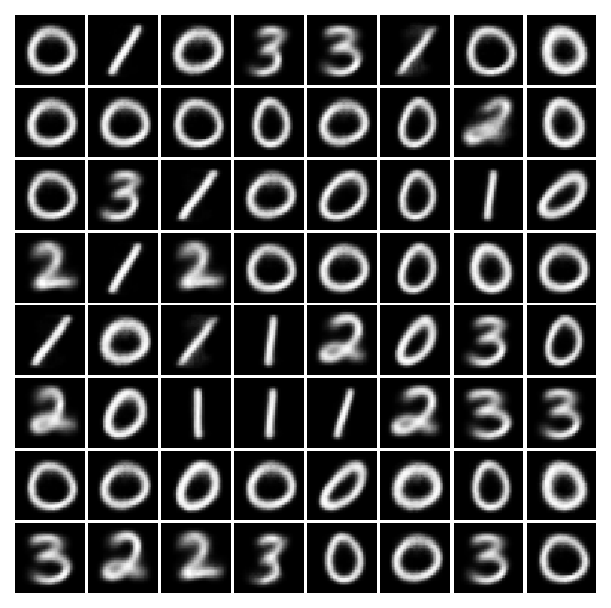
\includegraphics[scale=0.45]{latex/figures/samples_latent_dim_1_vanilla_conv_vae_bmnist.pdf}}}
\qquad
\subfloat[]{{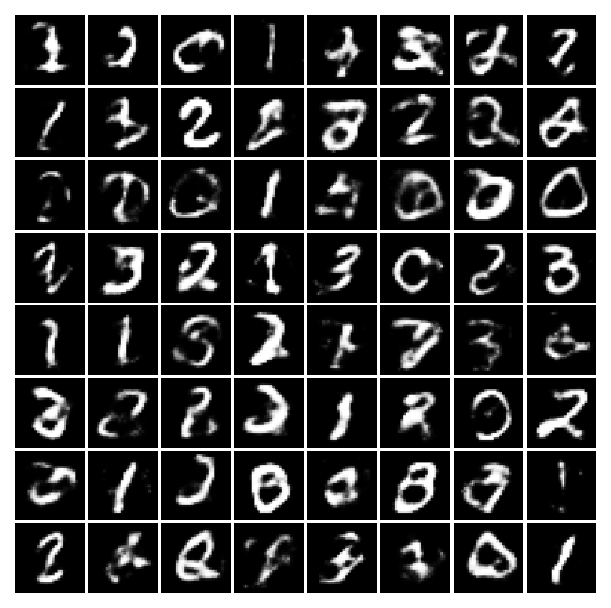
\includegraphics[scale=0.45]{latex/figures/samples_latent_dim_20_vanilla_mlp_vae_bmnist.pdf}}}
\qquad
\subfloat[]{{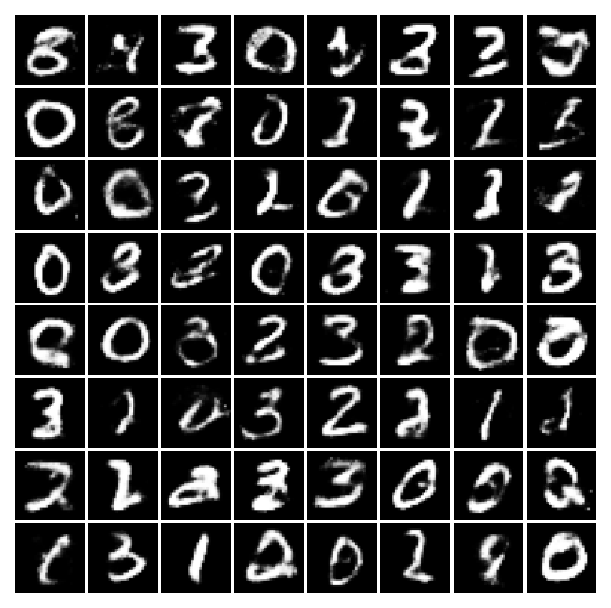
\includegraphics[scale=0.45]{latex/figures/samples_latent_dim_20_vanilla_dnn_vae_bmnist.pdf}}}
\qquad
\subfloat[]{{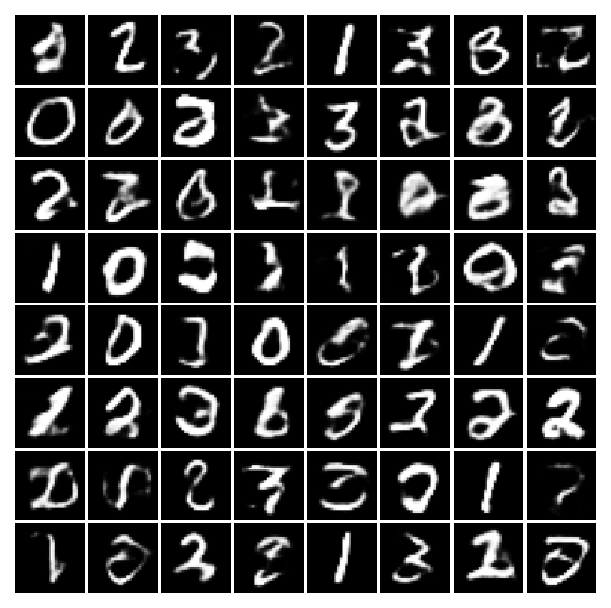
\includegraphics[scale=0.45]{latex/figures/samples_latent_dim_20_vanilla_conv_vae_bmnist.pdf}}}
\qquad
\subfloat[]{{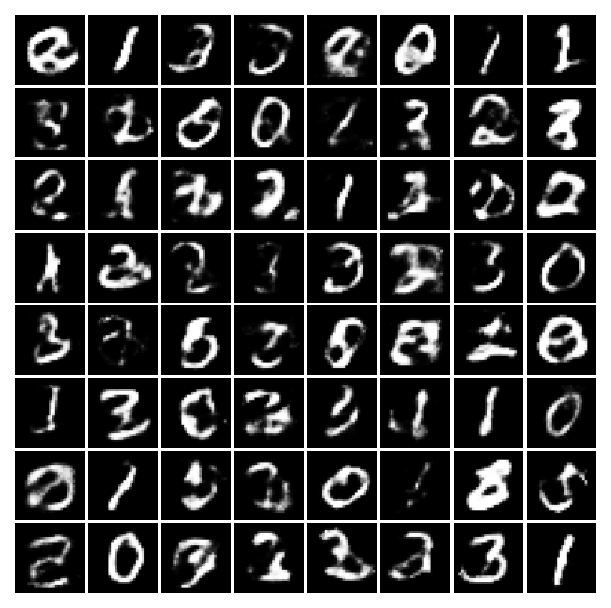
\includegraphics[scale=0.45]{latex/figures/samples_latent_dim_100_vanilla_mlp_vae_bmnist.pdf}}}
\qquad
\subfloat[]{{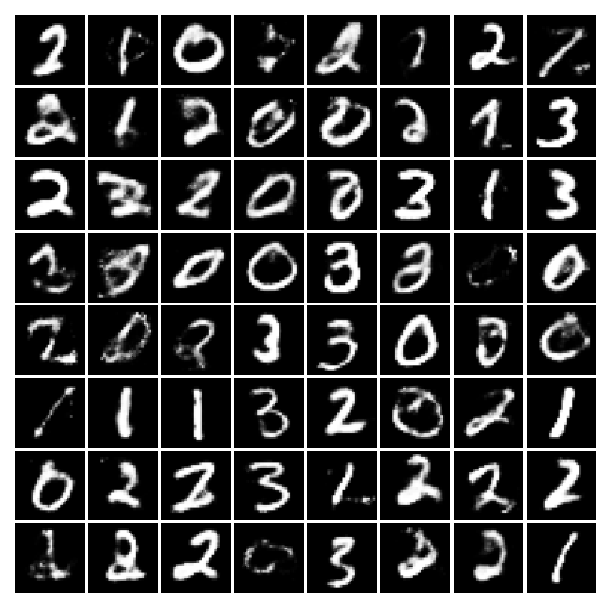
\includegraphics[scale=0.45]{latex/figures/samples_latent_dim_100_vanilla_dnn_vae_bmnist.pdf}}}
\qquad
\subfloat[]{{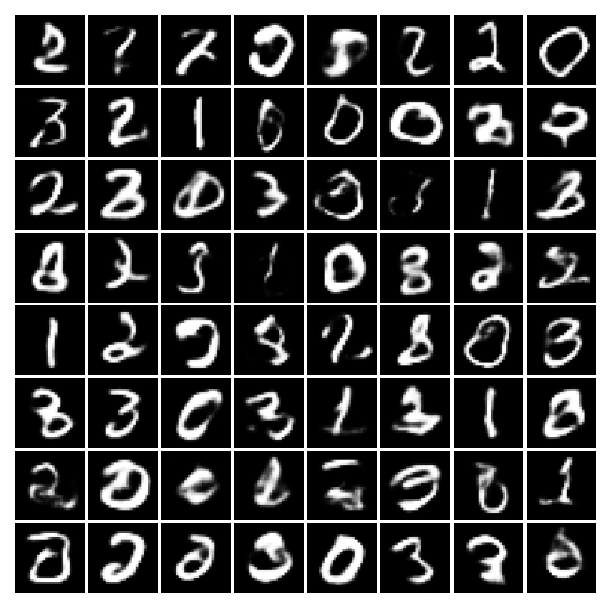
\includegraphics[scale=0.45]{latex/figures/samples_latent_dim_100_vanilla_conv_vae_bmnist.pdf}}}
\caption{Comparison of original and reconstructed images. Grids to the left are the MLP-VAE, in the middle DNN-VAE and to the right Conv-VAE. The top row shows 1 latent dimension, the middle 20 latent dimensions and the bottom 100}
\label{fig:samples_latent_dim_vanilla_vae_bmnist}
\end{figure}






\subsection{Disentangling the latent space}

\autoref{fig:tsne_beta_vae_bmnist} shows the t-SNE embedding of the latent distribution for different values of $\beta$. The color and label of each cluster corresponds to the MNIST digit label. .. on test set

\begin{figure}[!htb]
\centering
\subfloat[]{{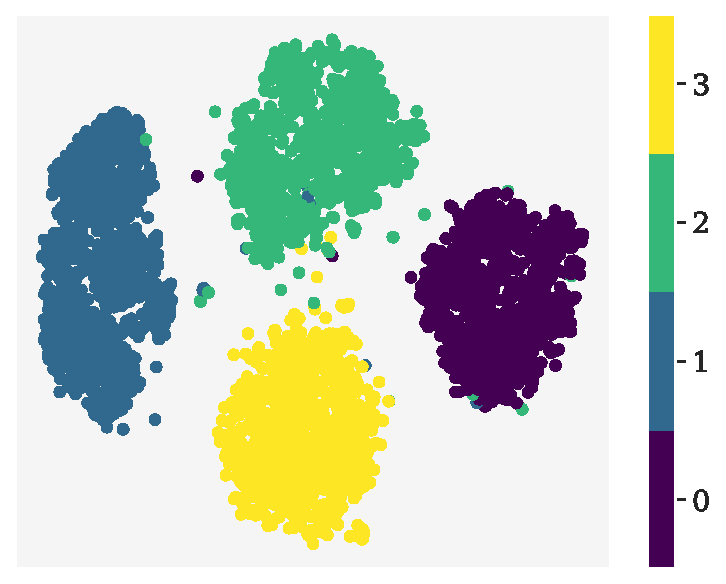
\includegraphics[scale=0.45]{latex/figures/tsne_beta_0.1_vae.pdf}}}
\qquad
\subfloat[]{{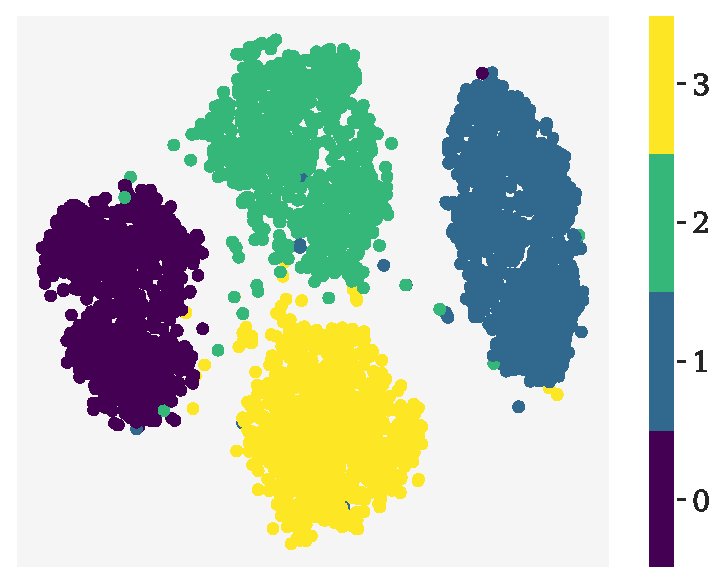
\includegraphics[scale=0.45]{latex/figures/tsne_beta_0.5_vae.pdf}}}
\qquad
\subfloat[]{{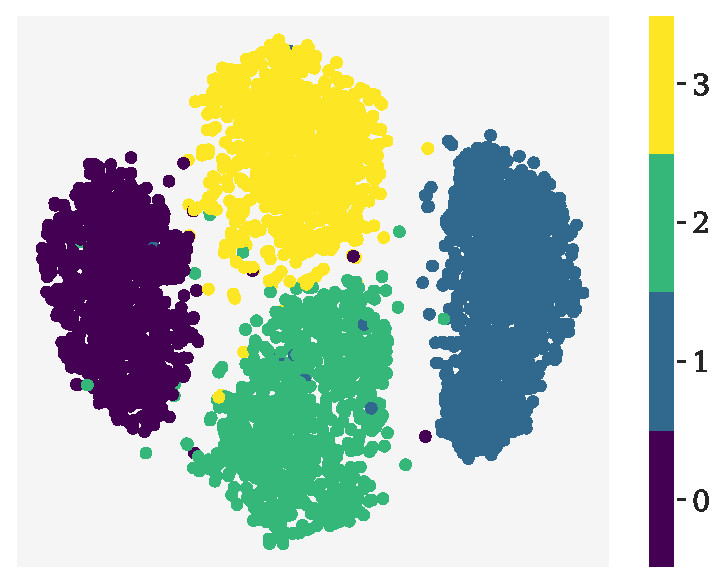
\includegraphics[scale=0.45]{latex/figures/tsne_beta_1_vae.pdf}}}
\qquad
\subfloat[]{{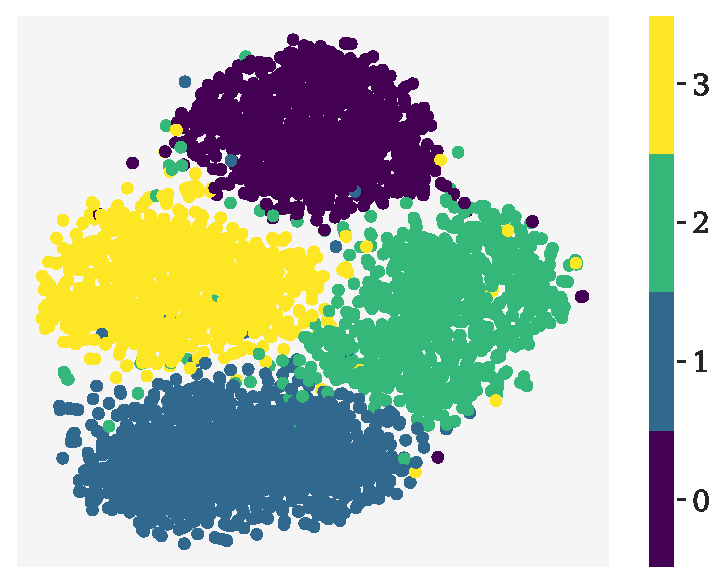
\includegraphics[scale=0.45]{latex/figures/tsne_beta_2_vae.pdf}}}
\qquad
\subfloat[]{{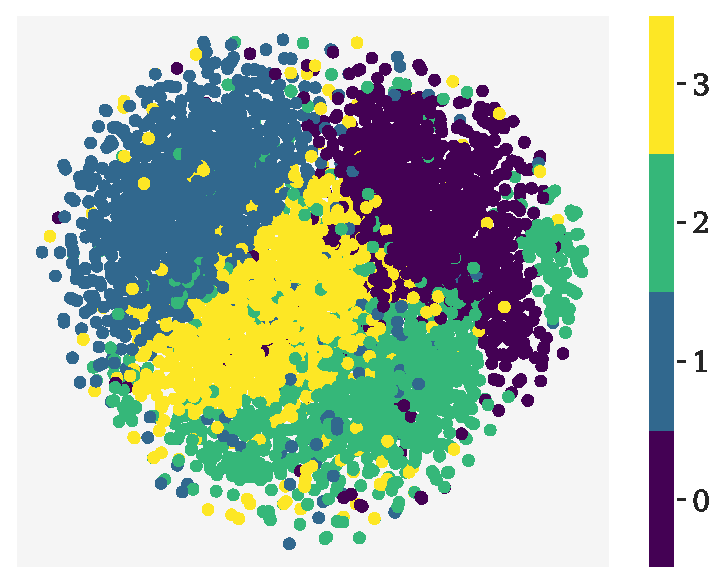
\includegraphics[scale=0.45]{latex/figures/tsne_beta_5_vae.pdf}}}
\qquad
\subfloat[]{{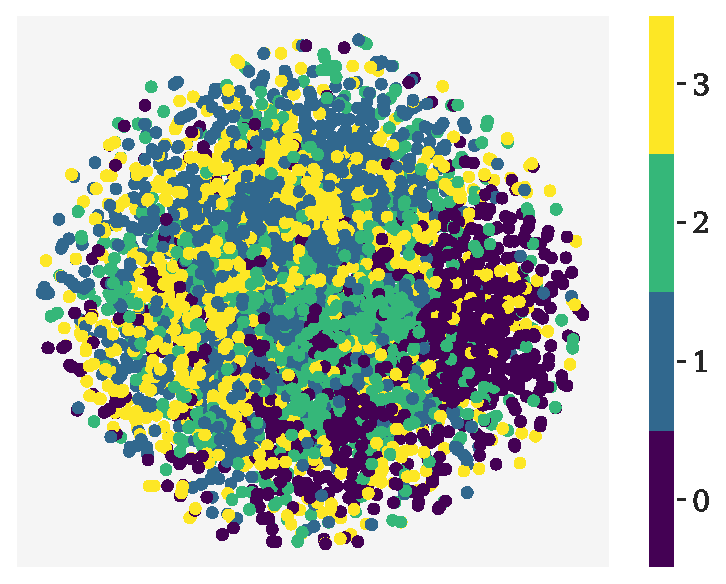
\includegraphics[scale=0.45]{latex/figures/tsne_beta_10_vae.pdf}}}
\caption{t-SNE }
\label{fig:tsne_beta_vae_bmnist}
\end{figure}


%----------------------------------------------------------------
\subsection{Results 1}\label{sec:project results}
%----------------------------------------------------------------

%\FloatBarrier


\url{https://uvadlc-notebooks.readthedocs.io/en/latest/tutorial_notebooks/JAX/tutorial9/AE_CIFAR10.html}

% Comparing latent dimensionality

% When training an autoencoder, we need to choose a dimensionality for the latent representation. The higher the latent dimensionality, the better we expect the reconstruction to be. However, the idea of autoencoders is to compress data. Hence, we are also interested in keeping the dimensionality low. To find the best tradeoff, we can train multiple models with different latent dimensionalities. The original input has 32x32x3 = 3072 pixels. Keeping this in mind, a reasonable choice for the latent dimensionality might be between 64 and 384:

% Clearly, the smallest latent dimensionality can only save information about the rough shape and color of the object, but the reconstructed image is extremely blurry and it is hard to recognize the original object in the reconstruction. With 128 features, we can recognize some shapes again although the picture remains blurry. The models with the highest two dimensionalities reconstruct the images quite well. The difference between 256 and 384 is marginal at first sight but can be noticed when comparing, for instance, the backgrounds of the first image (the 384 features model more of the pattern than 256).

% The encoder and decoder networks we chose here are relatively simple. Usually, more complex networks are applied, especially when using a ResNet-based architecture. For example, see VQ-VAE and NVAE